\documentclass[./\jobname.tex]{subfiles}
\begin{document}

\chapter{Experimental Design}
This chapter serves as an introduction to the experiments and gives an overview on how these are conducted. An integral part of solver comparison is to define a testbed that holds example problems with a known analytical solution. Further, quality measurements must be defined that compares the numerical to the analytical solution. The baseline for all experiments is the \gls{fem} solver NGSolve (\cite{mitchell_nist_2018}).

\section{Testbed}
The testbed is a collection of multiple different 2-dimensional scalar \gls{pde}s that are analytically solved such that $u(\mathbf{x}): \mathbf{R}^2 \rightarrow \mathbf{R}$ is a solution to the underlaying PDE. These can be used to demonstrate the correct implementation of a solver. The testbed can also be used to compare the performance of the classical \gls{fem} solver (NGSolve) with the \gls{ci} solver. The actual equations are displayed in the appendix \ref{chap:testbed}. The equations used here are a mixture of multiple different testbeds. Specifically, the equations 2 and 3 are picked from the testbed in \cite{chaquet_using_2019}. These problems were also used by \cite{tsoulos_solving_2006} and \cite{panagant_solving_2014}. Preliminary tests have shown that the equations used in these papers are rather simple to approximate. Thus, more complicate equations are added to test the solvability over a wider variety of functions. The more complex equations are taken from the National Institute of Standards and Technology (NIST) website (\cite{mitchell_nist_2018}) that provides benchmarking problems for \gls{fem} slovers with adaptive mesh refinement methods. The other equations 0A, 0B and 8 are specially created to show different properties of the solver. 

\textbf{PDE 0A: Gauss Kernel (equation \ref{eq:pde0a})} The analytic solution of this problem can be approximated arbitrarely close, since the solution is a sum of 5 different \gls{gak} as represented in equation \ref{eq:gauss_kernel}. The purpose of this PDE is to show that the algorithm converges towards the analytical solution. \\

\textbf{PDE 0B: GSin Kernel (equation \ref{eq:pde0b})} Similar to the PDE 0A, this problem is a sum of \gls{gsk}, as seen in equation \ref{eq:gsin_kernel}. To keep the search dimensionality roughly the same as in PDE 0A, the problem can be solved with 3 kernels. Again, the purpose of this equation is to determine the convergence with other kernel types.  \\

\textbf{PDE 1: Polynomial 2D (equation \ref{eq:pde1})} The solution of this equation is a polynomial of order 20. The function is 0 on the boundary of the unit square. (\cite{mitchell_nist_2018}) \\

\textbf{PDE 2: Chaquet PDE 1 (equation \ref{eq:pde2})} This is the problem of the Chaquet testbed, that is also used by several other authors. Its main purpose is to build the bridge to those papers so that the results can be compared. \cite{chaquet_using_2019} \\

\textbf{PDE 3: Chaquet PDE 3 (equation \ref{eq:pde3})} This equation is solved by a polynomial of order 2. Again, the purpose is to compare the results to other papers. \cite{chaquet_using_2019} \\

\textbf{PDE 4: Sine Bump 2D (equation \ref{eq:pde4})} The sine bump occures in a similar fashion in both, the Chaquet testbed (PDE 8 in \cite{chaquet_using_2019}) as well as the NIST (\cite{mitchell_nist_2018}) testbed. This means that the underlying solution function is the same, but the \gls{pde} is posed differently. Preliminary results have shown that the formulation of the NIST testbed is harder to solve. Thus, the formulation of Chaquet is disregarded and the NIST problem is implemented. \\

\textbf{PDE 5: Arctan Circular Wave Front (equation \ref{eq:pde5})} The main difficulty of this problem is the transition from the flat plateaus to the steep gradient of the circular wave front. Preliminary tests have shown that this equation is one of the most difficult problems in this testbed. (\cite{mitchell_nist_2018})\\

\textbf{PDE 6: Peak 2D (equation \ref{eq:pde6})} The solution to this problem is described by a single Gaussian ``peak'' at $(0.5, 0.5)$ with a large exponent. This solution could be approximated by a single \gls{gak}. The difficulty here is the steep gradient and a small region of interest. (\cite{mitchell_nist_2018})\\

\textbf{PDE 7: Boundary Line Singularity (equation \ref{eq:pde7})} This equation is only determined on $x \in \mathbf{R}^{+}$, which results in a singularity line at $x = 0$. Towards this line the gradient increases.  (\cite{mitchell_nist_2018})\\

\textbf{PDE 8: Interior Point Singularity (equation \ref{eq:pde8})} The idea of this \gls{pde} is similar to the problem 7, but the singularity is located on the inner domain. The solution to this problem is not defined at $(0.5, 0.5)$, resulting in a very difficult problem. \\

\textbf{PDE 9: Arctan Wave Front Homogeneous Boundary Conditions 2D (equation \ref{eq:pde9})} Similar to \gls{pde} 5, the difficulty of this problem is the steep gradient. Additionaly, the boundary condition is zero wich results in sharp corners on the boundary, that are hard to approximate. (\cite{mitchell_nist_2018})\\


\section{Software Architecture}

\definecolor{light-gray}{gray}{0.9}

\definecolor{testbed_colour}{RGB}{255,153,51}
\definecolor{opt_algo_colour}{RGB}{204,0,0}
\definecolor{kernels_colour}{RGB}{0,127,255}
\definecolor{post_proc_colour}{RGB}{198,41,255}

To simplify the preparation, execution and evaluation of the experiments, a comprehensive software architecture is defined. The \gls{uml} class diagram can be seen in the appendix \ref{chap:software_architecture}. The architecture is organised in 4 main segments. 

\textcolor{opt_algo_colour}{\large \underline{\textbf{optimisation algorithm in red}}} \\
The \colorbox{light-gray}{\lstinline[basicstyle=\ttfamily\color{black}]|IOptAlgoBase|} interface must be implemented by every \colorbox{light-gray}{\lstinline[basicstyle=\ttfamily\color{black}]|OptAlgo|} class to ensure the compatibility with \colorbox{light-gray}{\lstinline[basicstyle=\ttfamily\color{black}]|CiPdeBase|} class of the testbed. A nice side-effect is that it reduces the number of user-defined parameters. An optimisation algorithm of this class must only take an initial guess (e.g. the starting population) as well as two stopping criteria: the maximum number of function evaluation or a minimum error to reach. Also a fitness function (i.e. the function to be optimised) must be provided. Four lists of the same length are returned: the optimum-guess, the function value, the crossover probability and the scale factor per each generation. The actual implementation of the algorithm is not predefined. 

\textcolor{kernels_colour}{\large \underline{\textbf{kernels in blue}}} \\
As described in chapter \ref{chap:candidate_rep}, a candidate solution is defined as a sum of \gls{rbf}. In order to test different candidate representations, different classes must be implemented. Again, to ensure compatibility with the \colorbox{light-gray}{\lstinline[basicstyle=\ttfamily\color{black}]|CiPdeBase|} class, all representations must implement the \colorbox{light-gray}{\lstinline[basicstyle=\ttfamily\color{black}]|IKernelBase|} interface. This assures that all classes have a method that can calculate the solution as well as first and second order derivatives. Here, only two kernels are imlemented.

\textcolor{testbed_colour}{\large \underline{\textbf{testbed in orange}}} \\
The testbed holds the 11 differential equations used in all experiments. The testbed is abstraced in such a way that an experiment is as simple as creating an \gls{pde} object and calling its solve method. All testbed classes must implement the \colorbox{light-gray}{\lstinline[basicstyle=\ttfamily\color{black}]|ITestbenchBase|} interface. This ensures the minimal functionality of every subsequent class. Currently two classes implement this interface, the \colorbox{light-gray}{\lstinline[basicstyle=\ttfamily\color{black}]|FemPdeBase|} and the \colorbox{light-gray}{\lstinline[basicstyle=\ttfamily\color{black}]|CiPdeBase|}. These are the base classes that provide the specific attributes and methods needed for the \gls{fem} solver and the \gls{ci} solver. The actual \gls{pde} problems are implemented in the classes \colorbox{light-gray}{\lstinline[basicstyle=\ttfamily\color{black}]|FemPde0|} or \colorbox{light-gray}{\lstinline[basicstyle=\ttfamily\color{black}]|CiPde0|} which inherit from the \colorbox{light-gray}{\lstinline[basicstyle=\ttfamily\color{black}]|FemPdeBase|} and the \colorbox{light-gray}{\lstinline[basicstyle=\ttfamily\color{black}]|CiPdeBase|}, respectively. The number in their name is representative for all different testbench problems and every \gls{pde} has its own class. Since all \gls{pde} classes have the same methods and attributes and only differ in their implementation and name, they do not have to be displayed separately. Therefore, they are symbolised together by a ``stacked notation'' used in the class diagram. Some methods in these classes must be overridden and adapted to the current \gls{pde} problem, which is indicated by the $\land$ character.

\textcolor{post_proc_colour}{\large \underline{\textbf{post processing in purple}}} \\
Although the post processing block is not actually a class, it is still represented in this diagram. This module provides funtions that take \colorbox{light-gray}{\lstinline[basicstyle=\ttfamily\color{black}]|FemPdeN|} or \colorbox{light-gray}{\lstinline[basicstyle=\ttfamily\color{black}]|CiPdeN|} objects and performs actions with them. \todo{update implemented function description}

\begin{itemize}
	\item \colorbox{light-gray}{\lstinline[basicstyle=\ttfamily\color{black}]|bool saveExpObj(obj, filename)|} \\
	Save an \colorbox{light-gray}{\lstinline[basicstyle=\ttfamily\color{black}]|CiPdeN|} object as a \gls{json} file. The filename parameter can include a path, but it must end with .json. The results: execution time, memory usage, solution quality and all intergenerational data of the optimisation algoritm are stored in the file. 
	\item \colorbox{light-gray}{\lstinline[basicstyle=\ttfamily\color{black}]|dict loadExpObject(filename)|} \\
	Loads the \gls{json} file located at the specified filename, which again can include a path. A dictionary with the saved \colorbox{light-gray}{\lstinline[basicstyle=\ttfamily\color{black}]|CiPdeN|} parameters is returned. 
	\item \colorbox{light-gray}{\lstinline[basicstyle=\ttfamily\color{black}]|bool drawGaussKernel(parameter, ggb)|} \\
	Draws a solution approximated by Gauss kernels and with the specified parameters to a GeoGebra file. If the filename provided in the \textit{ggb} argument does not exist, the function searches for a template and prints to a copy of that file. 
	\item \colorbox{light-gray}{\lstinline[basicstyle=\ttfamily\color{black}]|bool drawGSinKernel(parameter, ggb)|} \\
	This is similar to the method drawGaussKernel method - but it takes parameters for a GSin kernel. 
	\item 
	\colorbox{light-gray}{\lstinline[basicstyle=\ttfamily\color{black}]|None plotApprox3D(kernel, parameter, lD, uD)|} \\
	The approximate solution of a \gls{pde} can be plotted over the with this function. Only square sized domains can be plotte, as specified by the lower and the upper domain parameters \textit{lD} and \textit{uD}. 
\end{itemize}

\section{Metric} 
\label{chap:metric}
In order to scientifically compare the results produced by the different solvers, some metrics are necessary. Three important solver-properties are measured: the execution time, the memory usage and the quality of the numerical solution. The following chapters describe the measurement process in greater detail. 

\subsection{Solving Time}
\label{chap:metric_time}
The solving time is measured within the \colorbox{light-gray}{\lstinline[basicstyle=\ttfamily\color{black}]|solve()|} method of either class. The time module of the \cite{python_standard_library_time_2020} is used to interact with the system clock. The resolution, that the time module can access, depends on the system it is running on. Specifically, on the machine used in all further experiments, \colorbox{light-gray}{\lstinline[basicstyle=\ttfamily\color{black}]|time.time()|} returns a 24 byte float that represents the time passed since 1st of January 1970. Usually, consecutive calls of this function return increasing values - changing the system time could interfere with the correctness of this value.\\ 

As the execution time of a program depends on many other factors, such as the current system load, the CPU temperature and the process scheduler, it is necessary to view it as a random variant. Thus, multiple replications have to be done before trying to interprete the results. These replications are not done within the \colorbox{light-gray}{\lstinline[basicstyle=\ttfamily\color{black}]|solve()|} function and must be applied during the experiment. To reduce the random effects and prevent possible outlier, the Python garbage collector is switched off during the time measurement. For a step-by-step description, the pseudocode is displayed in the appendix \ref{chap:solve_function}. 

\subsection{Memory Usage}
\label{chap:metric_mem}
Similar to the solving time measurement, the memory usage is determined within the \colorbox{light-gray}{\lstinline[basicstyle=\ttfamily\color{black}]|solve()|} method. The \textit{psutil} module (\cite{rodola_psutil_2020}) provides the functionality to read the amount of memory attached to a process at a given time. The function call \colorbox{light-gray}{\lstinline[basicstyle=\ttfamily\color{black}]|process.memory_info()|} returns an object with multiple attributes about the current state of the process. Of special interest is the \gls{vms} field. This includes the \gls{rss}, the memory that is currently held within the main memory, and the memory that is currently swapped out to the harddrive.

Without assuming anything about the inner workings of the process, the memory usage is also a random variant. Thus, similar to the time measurement, replications have to be performed. The same pseudocode as for the time measurement (appendix \ref{chap:solve_function}) also applies here. To remove outliers, it is helpfule to create and solve one testbed object before recording the experiment. This sets up the necessary references and which are then not mingled into the actual solving process. This holds true for both, the \gls{fem} and the \gls{ci} solver.  

\subsection{Quality Measurement}
\label{chap:metric_quality}
Although the fitness function is the criterion that is optimised, it is not applicable as an objective quality measure. As \cite{chaquet_using_2019} describe, it depends on multiple factors:
\begin{itemize}
	\item user-defined parameters $\xi$ and $\phi$ 
	\item the formulation of the \gls{pde} 
	\item number of collocation points used 
	\item number of kernels used
\end{itemize}
Thus, \cite{chaquet_using_2019} define a new quality measurement based on the \gls{rmse} over the collocation points as seen in equation \ref{eq:rmse_chaquet}. 
\begin{equation}
\label{eq:rmse_chaquet}
RMSE^2 = \frac{\sum_{i=1, \mathbf{x}_i \in C}^{n_C} \left|\left| \mathbf{u}(\mathbf{x}_i) - \mathbf{u_{ext}}(\mathbf{x}_i) \right|\right|^2 + \sum_{j=1, \mathbf{x}_j \in B}^{n_B} \left|\left| \mathbf{u}(\mathbf{x}_j) - \mathbf{u_{ext}}(\mathbf{x}_j) \right|\right|^2}{m(n_C + n_B)}
\end{equation}
This quality criterion has three inherent issues. At first, it firmly depends on the number of collocation points used. In an algorithm that uses self-adaptive collocation points, this measurement would be rendered useless. Further, the quality is only measured on the collocation points and not in between. However, a good solution fits not only these discrete points, but the whole domain. Finally, the \gls{fem} method doesn't use collocation points, so this quality measurement could not be calculated. A good quality measurement tool only uses the numerical and analytical solution, independently of the solving method. \\

This leads to the quality measurement formulation used in this thesis: the L2 norm defined for functions as denoted in equation \ref{eq:quality_measurement}. This actually measures the distance between the analytical solution and the numerical approximation.  
\begin{equation}
\label{eq:quality_measurement}
\left|\left|u_{ext} - u_{apx}\right|\right| = \sqrt{\int_{\Omega} (u_{ext}(\mathbf{x}) - u_{apx}(\mathbf{x}))^2 d\mathbf{x}}
\end{equation}
Although this integral is numerically evaluated, the discretisation is much finer than the resolution of the collocation points used in the fitness function - thus also regarding the areas between these points.



\section{Baseline: NGSolve}
As mentioned above, the NGSolve framework (\cite{schoberl_ngsolvengsolve_2020}) is used as the baseline for all experiments. NGSolve is a state of the art \gls{fem} solver, that is in part developed and maintained by numerous well-known institutes such as Vienna University of Technology, University of Göttingen and Portland State University. This chapter describes the results obtained by running NGSolve on the testbed. The metrics from chapter \ref{chap:metric} are applied. 

\subsection{Setup}
At first the \gls{pde}s must be transformed into their corresponding weak form. As all testbed problems are Poisson equations and only differ in their algebraic sign and inhomogeneous part, the weak form is similar for all problems. Refering to equation \ref{eq: weak form}, the terms $\vec{b} = 0$ and $c = 0$, thus these parts vanish. The matrix $A$ is either $\begin{bsmallmatrix} 1 & 0 \\ 0 & 1 \end{bsmallmatrix}$ or with a negative sign $\begin{bsmallmatrix} -1 & 0 \\ 0 & -1 \end{bsmallmatrix}$ as only the non-mixed second order derivatives occure in the equations. This results in weak form as presented in equation \ref{eq: weak form testbed}, where the f is the \gls{rhs} of the problem.
\begin{equation}
\label{eq: weak form testbed}
\int_{\Omega} \nabla u^T \nabla v dV = \int_{\Omega} f v dV
\end{equation}

To enhance the performance of NGSolve, static condensation is turned on. Further, a multigrid preconditioner is used. All problems are approximated by second order polynomials. The automatic mesh refinement is performed until a maximum of $5 \cdot 10^4$ \gls{dof} is reached. To properly interprete the results, 20 replications for each problem are performed. This is only needed for regarding time and memory, the solution itself is not a random variant. To further reduce the memory consumption, the GUI of NGSolve is switched off. 

\subsection{Result}
With the parameters described above, the following results are produced. The solving time as well as the memory usage are displayed in the boxplots \ref{fig:_fem_time_boxplot} and \ref{fig:_fem_mem_boxplot}, respectively. In general, the solving time ranges from 2.5 to 5.0 seconds at about 50 to 80 MByte of memory. Only problem 3 stands out as a notable exception. To keep the diagram visually appealing, this \gls{pde} is omitted and plotted in a separate figure. \\

The table \ref{tab:fem_sol_quality} presents the achieved distances between the exact and the approximated solutions. On \gls{pde} 3 the best numerical quality is achieved.\\

The problem \gls{pde} 7 only needs around 2.5 seconds to be solved. A reason could be that the solution only depends on one variable and the derivative with respect to y $\frac{\partial u}{\partial y} = 0$ vanishes. This does not effect the memory usage, since all $5 \cdot 10^4$ \gls{dof} must be created to terminate. 

\begin{table}[h]
	\centering
	\noindent\adjustbox{max width=\linewidth}{
		\begin{tabular}{|c|c|}
			
			\hline
			\rowcolor[HTML]{\farbeTabA}
			
			Problem PDE & Distance \\ \hline
			
			0A & $2.9670770746774782 \cdot 10^{-5}$ \\ \hline
			0B & $1.070854603999225 \cdot 10^{-5}$ \\ \hline
			1  & $8.004152462854497 \cdot 10^{-7}$ \\ \hline
			2  & $3.5013418621193666 \cdot 10^{-8}$ \\ \hline
			3  & $1.6795224037775289 \cdot 10^{-9}$ \\ \hline
			4  & $4.765830679060112 \cdot 10^{-7}$ \\ \hline
			5  & $6.056858428283682 \cdot 10^{-6}$ \\ \hline
			6  & $1.9078788449490833 \cdot 10^-{7}$ \\ \hline
			7  & $5.202739901395381 \cdot 10^{-5}$ \\ \hline
			8  & $3.237437258132996 \cdot 10^{-7}$ \\ \hline
			9  & $2.3655968008139198 \cdot 10^{-7}$ \\ \hline
			
		\end{tabular}
	}
	\unterschrift{These are the results obtained by the \gls{fem} solver in terms of distance to the analytical solution. The solver achieves the smallest deviation in PDE 3.}{}{}
	\label{tab:fem_sol_quality}
\end{table}


\begin{figure}[H]
	\centering
	\noindent\adjustbox{max width=0.66\linewidth}{
		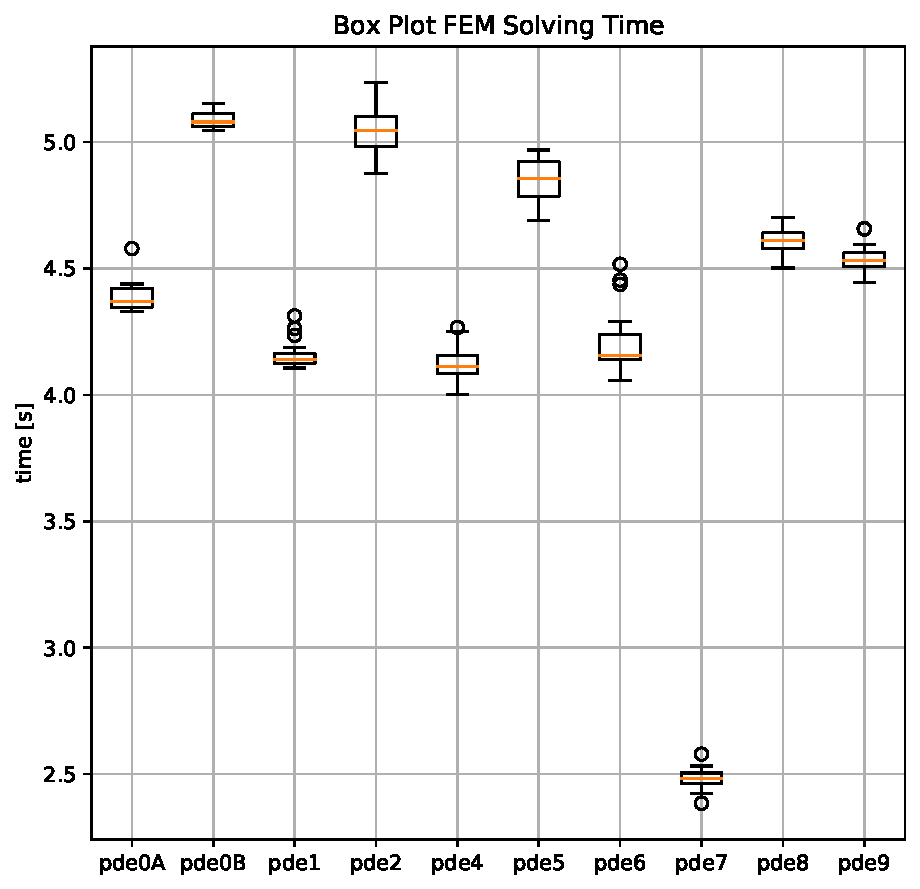
\includegraphics[width=\textwidth]{../../code/experiments/_experiment_fem_base/time_boxplot_pde_0a_0b_1_2_4_5_6_7_8_9.pdf}
	}
	\unterschrift{boxplot: time (in seconds) needed to solve the testbed \gls{pde} (without \gls{pde}3)}{}{}
	\label{fig:_fem_time_boxplot}
\end{figure}

\begin{figure}[H]
	\centering
	\noindent\adjustbox{max width=0.66\linewidth}{
		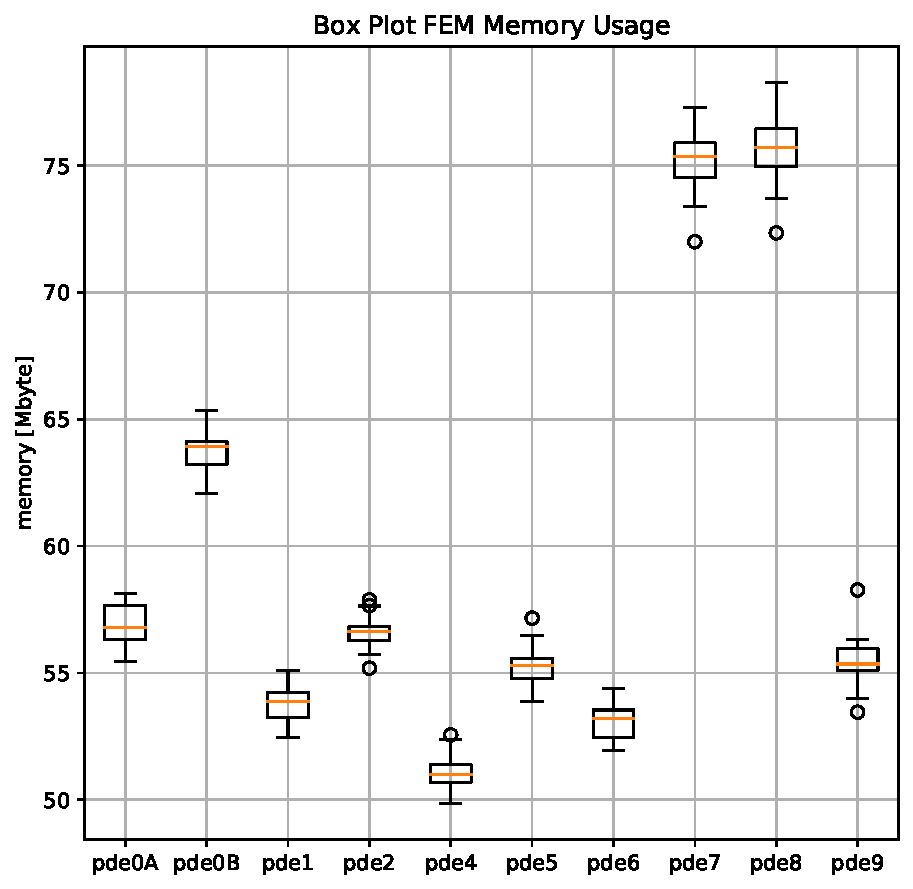
\includegraphics[width=\textwidth]{../../code/experiments/_experiment_fem_base/mem_boxplot_pde_0a_0b_1_2_4_5_6_7_8_9.pdf}
	}
	\unterschrift{boxplot: memory (in Mbyte) needed to solve the testbed \gls{pde} (without \gls{pde}3)}{}{}
	\label{fig:_fem_mem_boxplot}
\end{figure}

The following images \ref{fig:_fem_time_boxplot_pde3} and \ref{fig:_fem_mem_boxplot_pde3} show the boxplots of the time and memory consumption for the testbed \gls{pde} 3. Compared to the other equations, this problem takes longer to solve while also needing more memory: somewhere around 65.2 seconds at about 130 Mbyte. A possible explanation for that is the underlying structure of the \gls{pde}. As described in equation \ref{eq:sol3}, the exact solution to this problem is a polynomial of second order. This can be approximated perfectly by the \gls{fem} solver, since it also uses second order polynomials as basis functions. The mesh-refinement step takes more iteration to produce the $5 \cdot 10^4$ \gls{dof} as compared to the other testbed problems. 

\begin{figure}[H]
	\centering
	\noindent\adjustbox{max width=0.66\linewidth}{
		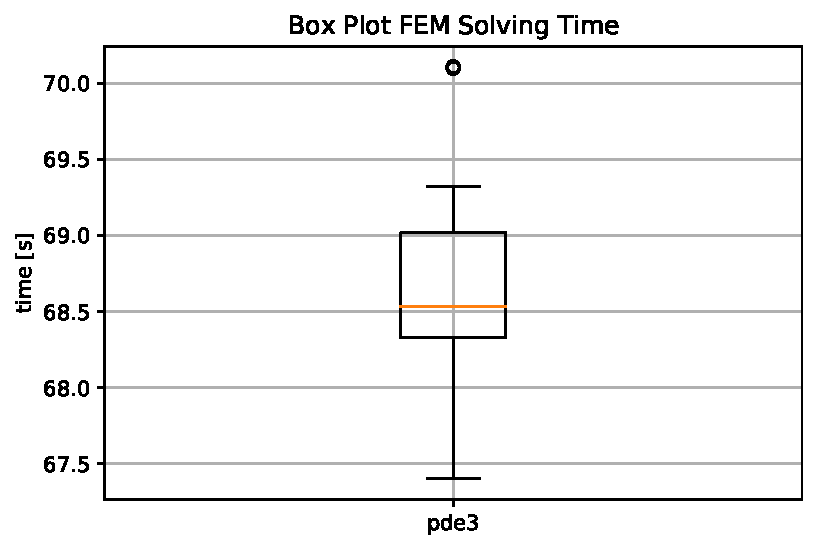
\includegraphics[width=\textwidth]{../../code/experiments/_experiment_fem_base/time_boxplot_pde_3.pdf}
	}
	\unterschrift{boxplot: time to solve testbed \gls{pde}3}{}{}
	\label{fig:_fem_time_boxplot_pde3}
\end{figure}

\begin{figure}[H]
	\centering
	\noindent\adjustbox{max width=0.66\linewidth}{
		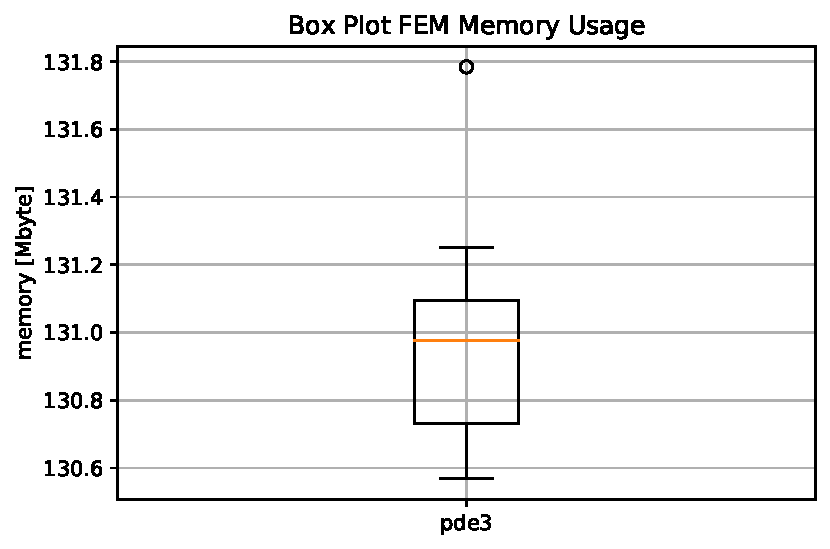
\includegraphics[width=\textwidth]{../../code/experiments/_experiment_fem_base/mem_boxplot_pde_3.pdf}
	}
	\unterschrift{boxplot: memory to solve testbed \gls{pde}3}{}{}
	\label{fig:_fem_mem_boxplot_pde3}
\end{figure}

\section{Default CI Parameter}
\label{chap:default_ci_param}

Typically, heuristic optimisation algorithm use some parameters to tune the performance on specific testbed problems - for all further experiments this is the JADE algorithm form pseudocode \ref{algo: jade}. Similary, the reported \gls{ci} solver has many parameters that could be adapted. However, adjusting every parameter in order to find the best combination is not an option, since that would take an extensive amount of computation time. Some parameters, that might not have a great effect on the performance, can be predefined. These values can be determined by preliminary tests or intuition, without any rigerous scientific justification. If not stated otherwise, the following parameters from table \ref{tab:ci_parameter} are used in the subsequent experiments. 

\begin{table}[h]
	\centering
	\noindent\adjustbox{max width=\linewidth}{
		\begin{tabular}{|c|c|c|}
			
			\hline
			\rowcolor[HTML]{\farbeTabA}
			
			Parameter & Value & Chaquet \\ \hline
			
			$\varphi$ & 100 & 300 \\ \hline
			$\kappa$  & 1   & 3   \\ \hline
			population size & $2 \cdot dim$ & $\frac{3}{2}(4 + \lfloor 3 \cdot ln(dim) \rfloor)$ \\ \hline
			min error & 0   & - \\ \hline
			p & 0.3 & - \\ \hline
			c & 0.5 & - \\ \hline
			replication & 20 & 50 \\ \hline
			\multilinecell{nb \\ nc \\~\\ } & \multilinecell{40 \\ 81 \\ \hline 121 = 11x11}  & \multilinecell{100 equally spaced \\ points over the domain} \\ \hline
			initialisation & $\vec{u_{apx}} \in \mathcal{N}(0,1)$ & \multilinecell{$\omega_i \in \mathcal{U}[-0.01, 0.01]$ \\ $\gamma_i \in \mathcal{U}(0,1]$ \\ $c_{ik} \in \mathcal{U}[2\Omega]$}  \\ \hline
			
		\end{tabular}
	}
	\unterschrift{These predefined parameters are used for the following numerical experiments. }{}{}
	\label{tab:ci_parameter}
\end{table}

The parameters $\varphi$ and $\kappa$ are used in the fitness function (equation \ref{eq:fit_func}) for changing the relative importance of the boundary and the interior. \cite{chaquet_using_2019} take similar values. However, preliminary tests have shown that the current values perform slightly better on the present testbed. Figure \ref{fig:collocation_points} shows the values of $\xi$ and $\varphi$. It further describes how the weighting factor emphasises the areas closer to the boundary. 

\begin{figure}[h]
	\centering
	\noindent\adjustbox{max width=0.75\linewidth}{
		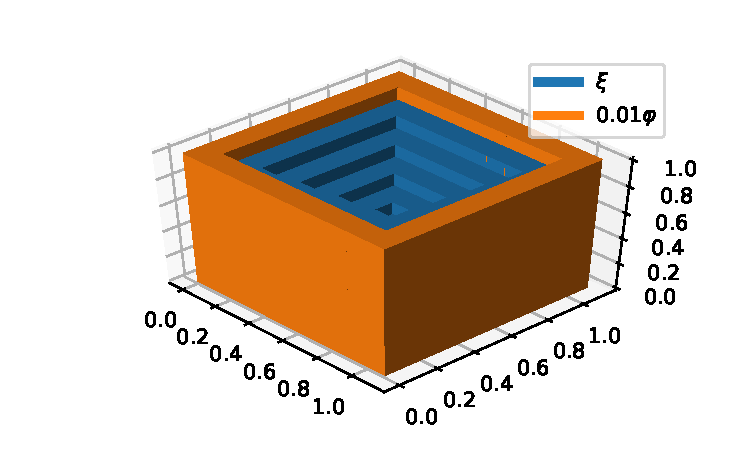
\includegraphics[width=\textwidth]{../img/pdf/collocation_weight.pdf}
	}
	\unterschrift{weighting factor $\varphi$ and $\xi$ on every collocation point}{}{}
	\label{fig:collocation_weight}
\end{figure}

The population size used by \cite{chaquet_using_2019} is based on the original formulation of the \gls{cma_es}. However, they observed a better convergence when scaling the recommended population size by 3. Typcially, \gls{de} uses larger population sizes. \cite{mallipeddi_empirical_2008} describe an empicial study on choosing this parameter. They discuss the tradeoff between premature convergence and computational effort. The results suggest that population sizes of $2\cdot dim$ do get stuck in local optimas, but also converge faster. Since time is a critical resource, this population size is chosen. 

The termination condition for \gls{de} is either a maximum number of function evaluation, or a minimal function value to reach. Since the fitness function (equation \ref{eq:fit_func}) has its optimum at 0, this value is used as the termination condition. A helpful side-effect is that it ensures the same amount of function evaluation in every run, without early termination. This prevents outliers in the time and memory measurement. 

The parameters p and c are specific to JADE (algorithm \ref{algo: jade}). The mutation operator \textit{mutationCurrentToPBest1} uses p to select the best individuals and c weights the parameter adaption mechanism. For all experiments these values are set at $p=0.3$ and $c=0.5$. 

To account for the statistical influence, all experiments are restarted 20 times with independant initial guesses. 

\cite{chaquet_using_2019} use 100 equally spaced collocation points over the domain to solve the \gls{pde}. Here, 121 points are created, as seen in figure \ref{fig:collocation_points}. 

\begin{figure}[h]
	\centering
	\begin{subfigure}[b]{0.5\linewidth}
		\centering
		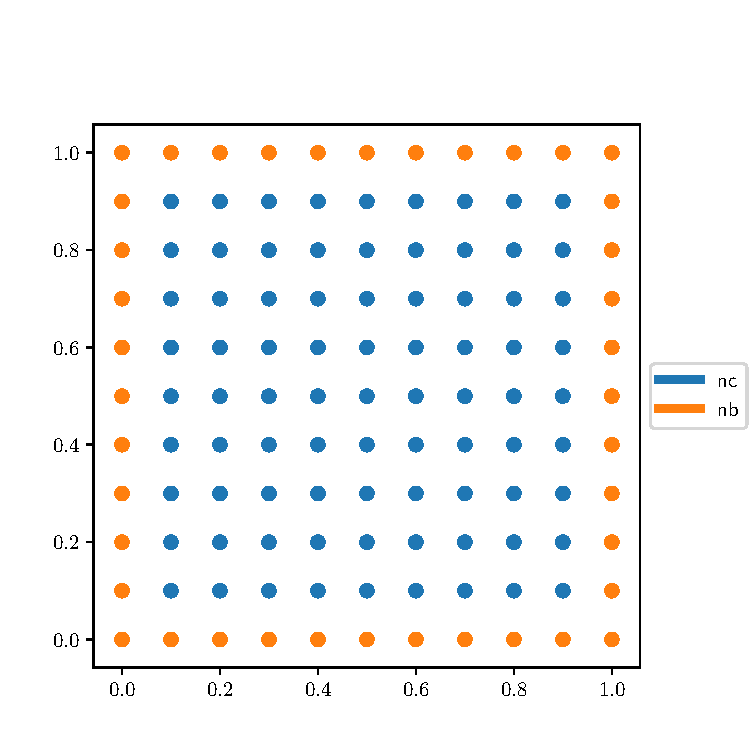
\includegraphics[width=1\textwidth]{../img/pdf/testbed_small_domain.pdf}
		\caption{collocation points on $\Omega: x\in [0,1]$}
		\label{fig:collocation_points_domain_small}
	\end{subfigure}% 
	%
	\begin{subfigure}[b]{0.5\linewidth}
		\centering
		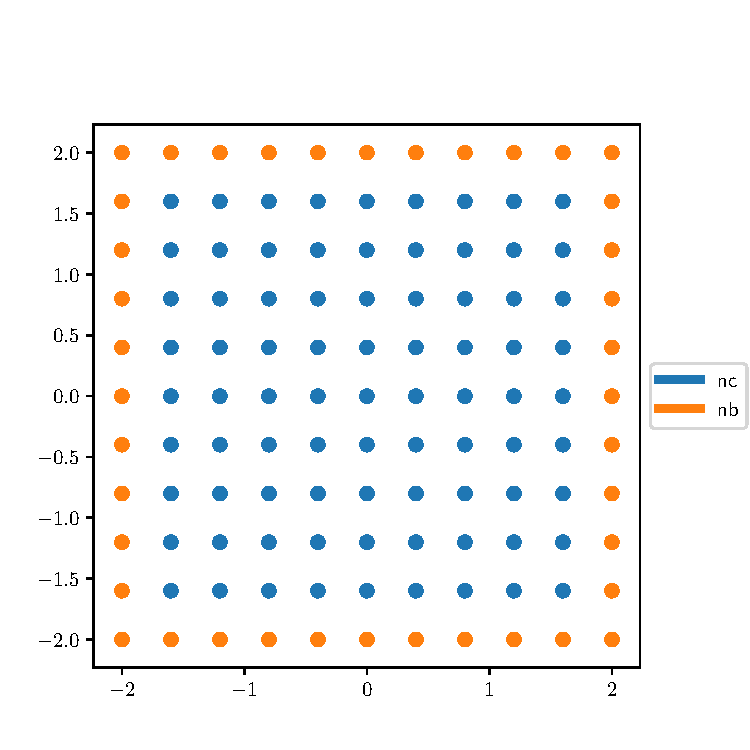
\includegraphics[width=1\textwidth]{../img/pdf/testbed_big_domain.pdf}
		\caption{collocation points on $\Omega: x\in [-2,2]$}
		\label{fig:collocation_points_domain_big}
	\end{subfigure}%
	\unterschrift{collocation points used on the two domains of the testbed}{}{}%
	\label{fig:collocation_points}
\end{figure}

The initialisation is done by a standard normal distribution. This means, that every value in the $\vec{u_{apx}}$ vector is drawn from a normal distribution. On the contrary, \cite{chaquet_using_2019} initialise the values specifically tailored to each parameter of the kernel. This process assumes a priori information about the solution and thus should be dropped. 



\end{document}